% Provenance (never printed): see sources/outline_sources.md (Year 2: anatexis, migmatites,
% granite types and their sources). Wet granite solidus from Stern and Wyllie (1981) and
% Boettcher and Wyllie (1968); dehydration-melting brackets from Patino Douce and Harris
% (1998), Berger and Kalt (1999), Skjerlie and Johnston (1996); water solubility from Holtz
% et al. (1995); migmatite terms from the IUGS-SCMR proposal and BGS RR 99-02; aluminosity
% after Shand (as given by Moyen et al. 2017); figure data in figdata/bachelor-2/anatexis.py
% (paths from ptpaths.py); exercise and problem values in the Book 4 scratch calculator
% calc/ch12.py.
\chapter{地壳熔融：混合岩与花岗岩}\label{ch:b2:crustal-melting}

花岗岩使大陆变轻，而地幔不能直接生成它：
\omterm{def:b2:mantle-melting:peridotites}{橄榄岩}的熔体是玄武岩。大部分花岗岩是大陆地壳自身熔融的产物。
当加厚的山根受热，当玄武岩在地壳下方聚积，或当炽热的岩石上升、压强降低时，
深部地壳中的云母和角闪石便失去其中的水，
晶粒之间出现花岗质液体，岩石变为\omterm{def:b2:crustal-melting:migmatite}{混合岩}，
一半变质、一半火成。本章追踪这种液体
从最初的薄膜，直至可能形成的\omterm{def:b2:magma-emplacement:bodies}{深成岩体}，
并从花岗岩的化学成分中读出它的母岩。

\begin{recall}
\textbf{来自高中分册}：花岗岩、花岗质岩和花岗闪长岩；长英质与镁铁质
岩石；造山带的根部。\textbf{来自本科一年级分册}：地壳中的放射性
生热；硅酸盐和黏土矿物的水解。\textbf{来自化学各册}：二元体系的固相线与液相线、
摩尔质量与物质的量。\textbf{来自
\cref{ch:b2:magma-emplacement}}：\omterm{def:b2:magma-emplacement:bodies}{岩墙}、\omterm{def:b2:magma-emplacement:bodies}{深成岩体}和\omterm{def:b2:magma-emplacement:ascent}{底辟}。\textbf{来自
\cref{ch:b2:mantle-melting}}：\omterm{def:b2:mantle-melting:melting}{部分熔融}、\omterm{def:b2:mantle-melting:peritectic}{不一致熔融}和\omterm{def:b2:mantle-melting:melting}{减压
熔融}。\textbf{来自\cref{ch:b2:metamorphic-facies}}：\omterm{def:b2:metamorphic-facies:protoliths}{变泥质岩}、反应的\omterm{def:b2:metamorphic-facies:clapeyron}{克拉珀龙斜率}
和\omterm{def:b2:metamorphic-facies:facies}{变质相}。\textbf{来自\cref{ch:b2:pt-paths}}：\omterm{def:b2:pt-paths:ptt}{P--T--t 轨迹}和
地壳增厚模型。
\end{recall}

\section{地壳为何熔融}\label{sec:b2:crustal-melting:why}

这个词古老而朴素。

\begin{definition}[深熔作用]\label{def:b2:crustal-melting:anatexis}
\emph{深熔作用}\index{深熔作用}是岩石的熔融，无论熔融程度如何；
实际上该词专指大陆地壳的\omterm{def:b2:mantle-melting:melting}{部分熔融}。
\end{definition}
% ledger: scmr:migmatite

\subsection*{湿固相线}

花岗岩只有含水时才会在较低温度下熔化。斯特恩和怀利
用过量水熔化了一块取自内华达山脉\omterm{def:b2:magma-emplacement:bodies}{岩基}的黑云母花岗岩：首个液相出现的温度，
在\qty{2}{kbar}时为\qty{680}{\celsius}，在\qty{10}{kbar}时为\qty{620}{\celsius}，而整块岩石
在\qty{2}{kbar}下仅高出固相线\qty{35}{\celsius}即全部熔化，而
在\qty{10}{kbar}下则高出固相线\qty{105}{\celsius}。先前研究的同一花岗岩，
由伯切尔和怀利研究，在\qty{15.3}{kbar}下于\qty{605}{\celsius}开始熔化；在约
\qty{17}{kbar}时，斜长石分解为硬玉与石英，此后固相线
转而上升，在\qty{27}{kbar}时达到\qty{670}{\celsius}。
% ledger: sw81:wet-solidus, bw68:wet-solidus

湿固相线随压强升高而下降，与干固相线的行为相反。原因在于
水的去向。自由水是低密度流体，溶入熔体后所占体积很小：
霍尔茨等人测得其在花岗质熔体中的偏摩尔体积接近
\qtyrange{10}{12}{\cubic\centi\metre\per\mole}，而室温下液态水为
\qty{18}{\cubic\centi\metre\per\mole}，热流体则更大。熔融反应写作
\[\text{石英} + \text{长石} + \ce{H2O}\ (\text{流体}) \longrightarrow
\text{含水熔体}\]
因此该反应的体积变化为负，熵变则与任何熔融一样为
正：由\cref{ch:b2:metamorphic-facies}中的克拉珀龙关系，其斜率
$\mathrm{d}P/\mathrm{d}T = \Delta S/\Delta V$ 为负。压强还使更多的水
进入熔体：对于\qty{800}{\celsius}下的简单花岗质熔体，饱和含水量
在\qty{0.5}{kbar}时质量分数为\qty{2.80}{\percent}，在\qty{5}{kbar}时为\qty{9.97}{\percent}，
在\qty{8}{kbar}时为\qty{13.82}{\percent}；在 3 至\qty{8}{kbar}之间，
每\unit{kbar}约多溶\qty{1.27}{\percent}。
% ledger: holtz95:solubility

\begin{omfigure}
\centering
\begin{tikzpicture}
\begin{axis}[omrecord, width=0.5\linewidth, height=4.8cm,
  xmin=0, xmax=9, ymin=0, ymax=15, xlabel={$P$ (\unit{kbar})},
  ylabel={熔体中的 \ce{H2O} (\unit{\percent})},
  tick label style={font=\scriptsize}, label style={font=\small}]
\addplot[only marks, mark=*, mark size=1.6pt, blue!70!black]
  table[x=P_kbar, y=H2O_wt] {figdata/out/bachelor-2-anatexis-water.dat};
\addplot[thick, red!75!black] table[x=P_kbar, y=H2O_wt] {figdata/out/bachelor-2-anatexis-waterfit.dat};
\end{axis}
\end{tikzpicture}
\par\smallskip{\small 简单花岗质熔体在\qty{800}{\celsius}下能溶解的水
（实测点）；红线为过 3 至
\qty{8}{kbar}各点的最小二乘直线，斜率为\qty{1.26}{\percent}每\unit{kbar}。}
\end{omfigure}
% ledger: holtz95:solubility

但深部地壳几乎没有自由水：一块经过加热的变质岩，
已经通过
\cref{ch:b2:metamorphic-facies}中的脱水反应驱出了大部分孔隙水。其水分现锁存于云母和角闪石中，熔融
则须等待这些矿物本身分解。

\begin{definition}[流体参与熔融与脱水熔融]\label{def:b2:crustal-melting:reactions}
\emph{流体参与熔融}\index{流体参与熔融}（或称水助熔融）是
在有自由含水流体存在、位于或接近湿固相线处发生的熔融；所产生的熔体
其量受流体供应限制。\emph{脱水熔融}\index{脱水熔融}
（无流体熔融）是含水矿物（云母或角闪石）与石英、长石共同发生的\omterm{def:b2:mantle-melting:peritectic}{不一致熔融}，
无任何自由流体参与：矿物中的水
进入熔体，并生成新的无水矿物（包晶钾长石、铝硅酸盐、
石榴子石、堇青石、斜方辉石）在其旁生长。
\end{definition}
% ledger: pj98:productivity, koester02:melting, pdh98:himalaya

实验确定了各含水矿物在何处分解。在取自喜马拉雅的白云母片岩中，
帕蒂尼奥·杜塞和哈里斯发现，\omterm{def:b2:crustal-melting:reactions}{脱水熔融}始于 750 至
\qty{800}{\celsius}，压强为 6 至\qty{10}{kbar}；向同一岩石加水，固相线下降，
但所产生的是奥长花岗质熔体，与\omterm{def:b2:crustal-melting:leucogranite}{淡色花岗岩}不同。一块半泥质片麻岩
在约\qty{700}{\celsius}时借其多硅白云母开始熔化，但熔体产量
不足\qty{9}{\percent}；超过\qty{800}{\celsius}后，黑云母与堇青石分解，
按体积计产生 10 至\qty{63}{\percent}的熔体。黑云母\omterm{def:b2:crustal-melting:reactions}{脱水熔融}
在 800 至\qty{850}{\celsius}、0.5 至\qty{0.7}{GPa} 条件下发生于巴伐利亚森林的\omterm{def:b2:crustal-melting:migmatite}{混合岩}中，
而角闪石按体积计增加约\qty{25}{\percent}的熔体，温度为 875 至
\qty{925}{\celsius}，压强为 10 至\qty{12.5}{kbar}。次序取决于水被束缚的程度：
白云母最先，黑云母其次，角闪石最后。
% ledger: pdh98:himalaya, koester02:melting, bk99:migmatites, sj96:amphibole, moyen17:aluminosity

\begin{proposition}[受水量限制的熔体分数]\label{prop:b2:crustal-melting:water}
在无游离流体的\omterm{def:b2:crustal-melting:reactions}{脱水熔融}中，若一块岩石含有质量分数为 $X$ 的某种
含水矿物，其中水的质量分数为 $w$，且全部水进入一个
含水质量分数为 $c$ 的熔体，则熔体的质量分数为
\[F = \frac{X\,w}{c}.\]
由于 $c$ 不能超过熔融时压强和温度下的饱和含水量 $c_{\mathrm{sat}}$，
故 $F \ge X\,w/c_{\mathrm{sat}}$：熔体含水越少，
同一云母生成的熔体就越多。
\end{proposition}

\begin{proof}
每千克岩石中，矿物释放 $X\,w$ 千克水。无游离流体相，
固体中也不剩水，全部水都进入熔体。熔体质量为 $F$，其中含水 $c\,F$
千克：$c\,F = X\,w$。由于 $c \le c_{\mathrm{sat}}$，$F = Xw/c \ge
Xw/c_{\mathrm{sat}}$。
\end{proof}

白云母 \ce{KAl3Si3O10(OH)2}，摩尔质量为 \qty{398.3}{\gram\per\mole}，含有两个
羟基，相当于一个水分子，即占其质量的 \qty{4.52}{\percent}。
因此，含 \qty{20}{\percent} 白云母的片岩每千克可释放 \qty{9.0}{\gram} 水，
若以 \qty{6}{\percent} 的含水量溶解，可生成 \qty{150}{\gram}
熔体。云母决定了水的预算，因此易熔地壳，
即最易熔化的地壳，富含云母，其中\omterm{def:b2:metamorphic-facies:protoliths}{变泥质岩}最为突出。

\begin{omfigure}
\centering
\begin{tikzpicture}
\begin{axis}[omrecord, width=0.8\linewidth, height=7cm,
  xmin=500, xmax=1000, ymin=0, ymax=20, xlabel={$T$ (\unit{\celsius})}, ylabel={$P$ (\unit{kbar})},
  tick label style={font=\scriptsize}, label style={font=\small}, clip=false]
\addplot[fill=orange!35, draw=orange!70!black] coordinates {(750,6) (800,6) (800,10) (750,10) (750,6)};
\addplot[fill=red!25, draw=red!70!black] coordinates {(800,5) (850,5) (850,7) (800,7) (800,5)};
\addplot[fill=green!25, draw=green!50!black] coordinates {(875,10) (925,10) (925,12.5) (875,12.5) (875,10)};
\node[font=\scriptsize, orange!50!black, align=center] at (axis cs:775,8) {白云母};
\node[font=\scriptsize, red!60!black] at (axis cs:825,4.4) {黑云母};
\node[font=\scriptsize, green!35!black, anchor=west] at (axis cs:927,11.25) {角闪石};
\addplot[very thick, blue!70!black, mark=*, mark size=1.5pt]
  table[x=T_C, y=P_kbar] {figdata/out/bachelor-2-anatexis-solidi.dat};
\node[font=\scriptsize, blue!70!black, anchor=west] at (axis cs:612,15.6) {含水花岗岩固相线};
\addplot[thick, black, postaction={decorate}, decoration={markings,
  mark=at position 0.3 with {\arrow{>}}, mark=at position 0.75 with {\arrow{>}}}]
  table[x=T_C, y=P_kbar, restrict x to domain=500:1000,
  restrict expr to domain={\thisrow{t_Myr}}{0:100}] {figdata/out/bachelor-2-anatexis-path35.dat};
\node[font=\scriptsize, anchor=north] at (axis cs:560,4.2) {起始深度 \qty{35}{km} 的岩石};
\addplot[thick, dashed, black, postaction={decorate}, decoration={markings,
  mark=at position 0.3 with {\arrow{>}}, mark=at position 0.7 with {\arrow{>}}}]
  table[x=T_C, y=P_kbar, restrict x to domain=500:1000,
  restrict expr to domain={\thisrow{t_Myr}}{0:100}] {figdata/out/bachelor-2-anatexis-path70.dat};
\node[font=\scriptsize, anchor=south] at (axis cs:760,19.4) {加厚地壳底部};
\end{axis}
\end{tikzpicture}
\par\smallskip{\small 地壳在何处熔融。蓝色：含过量水的黑云母花岗岩固相线
（实测点，以直线段相连）。方框：白云母、黑云母与角闪石\omterm{def:b2:crustal-melting:reactions}{脱水熔融}在实验
和\omterm{def:b2:crustal-melting:migmatite}{混合岩}中被观测到的条件。黑色：由\cref{ch:b2:pt-paths}中的加厚模型
算得的路径：堆叠后最终位于 \qty{35}{km} 深处的岩石（实线）始终未达湿固相线，
而加厚地壳底部（虚线）经过
\qty{900}{\celsius}。两条路径均只画出前
1 亿年，直至
侵蚀停止为止。}
\end{omfigure}
% ledger: sw81:wet-solidus, bw68:wet-solidus, pdh98:himalaya, bk99:migmatites, sj96:amphibole, et84:ptt

\subsection*{热量从何而来}

上图提出了问题：地壳只有在高于约
\qty{700}{\celsius}时才会熔融，而在\cref{ch:b2:pt-paths}中的模型里，稳定地温线
在 \qty{35}{km} 厚地壳的底部仅达 \qty{595}{\celsius}。有三种途径
可越过\omterm{def:b2:crustal-melting:reactions}{脱水熔融}反应。

\emph{加厚与放射性生热。}在\cref{ch:b2:pt-paths}中的模型里，经堆叠而加倍的地壳
从内部升温；止于地壳中部深度的岩石峰值温度为 \qty{593}{\celsius}，从未熔融，
但加厚地壳的底部在约 3100 万年后超过 \qty{800}{\celsius}，
约 5600 万年后超过 \qty{900}{\celsius}，已超出黑云母反应的范围。
下地壳的熔融是加厚的缓慢后果。
% ledger: et84:ptt

\emph{\omterm{def:b2:mantle-melting:melting}{减压熔融}。}一块热岩石被抬升的速度快于其冷却速度，从高压一侧
越过\omterm{def:b2:crustal-melting:reactions}{脱水熔融}曲线。帕蒂尼奥·杜塞和哈里斯发现，白云母片岩的固相线
的 $\mathrm{d}P/\mathrm{d}T$ 比黑云母片岩的更小，
故白云母片岩在减压时更易熔融；他们断定，
喜马拉雅\omterm{def:b2:crustal-melting:leucogranite}{淡色花岗岩}由\omterm{def:b2:metamorphic-facies:protoliths}{变泥质岩}\omterm{def:b2:crustal-melting:reactions}{脱水熔融}形成，
发生于绝热减压过程中，压强为 6 至 \qty{8}{kbar}，温度为 750 至 \qty{770}{\celsius}。
% ledger: pdh98:himalaya

\emph{来自下方的热量。}止于地壳底部的地幔玄武岩带来
它携带的热量和结晶潜热。

\begin{definition}[镁铁质底侵]\label{def:b2:crustal-melting:underplating}
\emph{镁铁质底侵}\index{镁铁质底侵}是指源自地幔的
玄武质\omterm{def:b2:magma-emplacement:magma}{岩浆}在陆壳底部或其附近滞留，并在其中结晶，
把热量释放给上覆地壳。
\end{definition}

例如，曾用底侵作用解释南极半岛的流纹岩，
其母\omterm{def:b2:magma-emplacement:magma}{岩浆}为安山质至英安质，来自含水镁铁质下地壳在底侵作用
下的熔融；地幔熔体本身也可以形成花岗岩类，
即通过结晶，或重熔新近底侵的岩体。
% ledger: riley01:underplating, moyen17:settings, johansson23:a-type

\begin{proposition}[底侵的热量收支]\label{prop:b2:crustal-melting:heat}
体积为 $V_b$、温度为 $T_b$ 的玄武岩侵入后完全结晶，释放出
单位体积潜热 $L_b$，并冷却至 $T_f$，能使体积为 $V_c$ 的地壳
由 $T_c$ 升至 $T_f$，并使其中比例为 $F$ 的\omterm{def:b2:mantle-melting:melting}{部分熔融}，此时有
\[\frac{V_c}{V_b} = \frac{L_b + C\,(T_b - T_f)}{C\,(T_f - T_c) + F\,L_c},\]
其中 $C$ 为单位体积热容（两种岩石取相同值），$L_c$ 为
地壳熔体单位体积的潜热，设无热量损失。
\end{proposition}

\begin{proof}
玄武岩释放的热量 $V_b[L_b + C(T_b - T_f)]$，等于
地壳吸收的热量 $V_c[C(T_f - T_c) + F L_c]$；两边同除以 $V_b$，并除以地壳项中的方括号。
\end{proof}

取 $C = \qty{2.5}{\mega\joule\per\cubic\metre\per\kelvin}$，潜热为
\qty{900}{\mega\joule\per\cubic\metre}（均为\omterm{def:b2:magma-emplacement:magma}{岩浆}的典型值），一块由
\qty{1200}{\celsius} 冷却至 \qty{850}{\celsius} 的玄武岩，可使约两倍半于自身体积的
地壳由 \qty{650}{\celsius} 升温，并使其五分之一熔融（见\cref{exo:b2:crustal-melting:7}）。
底侵效率很高，但具有局地性：热量只流向玄武岩所在之处。
% ledger: delaney86b4:properties

\section{深熔作用与混合岩}\label{sec:b2:crustal-melting:migmatites}

\omterm{def:b2:mantle-melting:melting}{部分熔融}的岩石，若在熔体离开之前便已凝固，则其两部分会并列保存下来。

\begin{definition}[混合岩及其组成部分]\label{def:b2:crustal-melting:migmatite}
\emph{混合岩}\index{混合岩}是一种复合硅酸盐岩石，在露头尺度上
不均一，由较暗的部分和较浅的部分组成，较暗部分具有变质岩的外观，较浅部分
具有深成岩的外观。其\emph{浅色体}\index{浅色体}为较亮的部分，富含石英和
长石；其\emph{暗色体}\index{暗色体}为暗色部分，富含暗色矿物，
与浅色体互补；其\emph{中色体}为中间颜色的部分，
即\omterm{def:b2:metamorphic-facies:metamorphism}{原岩}或多或少经改造的残留体（\emph{古成体}）。浅色体与
暗色体共同组成\emph{新成体}，即新形成的部分。
\emph{变熔混合岩}\index{变熔混合岩}是一种具有分立、界线清楚的浅色体、中色体和暗色体的混合岩；
\emph{深熔混合岩}\index{深熔混合岩}则是浅色与暗色部分
在条纹（条带）与幽灵状（云状）构造中相互融合的混合岩。
\end{definition}
% ledger: scmr:migmatite, bgs99:migmatite

该定义刻意保持描述性：\omterm{def:b2:crustal-melting:migmatite}{浅色体}是否为凝固的熔体、来自别处的熔体，
还是变质分异作用的产物，属于一种解释。若其为熔体，
则\omterm{def:b2:crustal-melting:migmatite}{浅色体}为液相，\omterm{def:b2:crustal-melting:migmatite}{暗色体}为其所遗留的固体残留物，富含
黑云母、石榴子石或堇青石：\omterm{def:b2:crustal-melting:migmatite}{变熔混合岩}记录了\omterm{def:b2:crustal-melting:anatexis}{深熔作用}的初始阶段，此时
只有部分岩石熔化；\omterm{def:b2:crustal-melting:migmatite}{深熔混合岩}则代表\omterm{def:b2:crustal-melting:anatexis}{深熔作用}的晚期阶段，此时暗色矿物也已熔化，
且熔体仍留在原地。
% ledger: scmr:migmatite

\omterm{def:b2:crustal-melting:migmatite}{混合岩}中熔体含量有多少？在巴伐利亚森林的堇青石\omterm{def:b2:crustal-melting:migmatite}{混合岩}中，
由黑云母\omterm{def:b2:crustal-melting:reactions}{脱水熔融}形成、纯属原先熔体的\omterm{def:b2:crustal-melting:migmatite}{浅色体}，按体积计占岩石的 20 至
\qty{40}{\percent}，与相同条件下对类似岩石进行\omterm{def:b2:crustal-melting:reactions}{脱水熔融}实验所得的 20 至 \qty{30}{\percent} 相近；
而在变形最强的类型中，熔体已被排出，
残留的岩石则留存下来。
% ledger: bk99:migmatites

\begin{inthefield}[读解混合岩露头]
在\omterm{def:b2:crustal-melting:migmatite}{混合岩}露头上，地质学家首先描绘各部分及其几何形态：\omterm{def:b2:crustal-melting:migmatite}{浅色体}位于面理之中还是
切穿面理，是否带有暗色的边缘，
以及每个\omterm{def:b2:crustal-melting:migmatite}{浅色体}对应多少\omterm{def:b2:crustal-melting:migmatite}{暗色体}。每一特征都有其意义。残留的、
暗色的岩石标示熔体的来源；细小、短促、分叉的\omterm{def:b2:crustal-melting:migmatite}{浅色体}
伴随的\omterm{def:b2:crustal-melting:migmatite}{暗色体}很少，标示熔融刚刚开始；与面理平行的\omterm{def:b2:crustal-melting:migmatite}{浅色体}
标示熔体从基质中排出并在此聚集；与层理成大角度的\omterm{def:b2:crustal-melting:migmatite}{浅色体}
通常没有暗色边缘，形成最晚，标示熔体离开的
通道。\omterm{def:b2:crustal-melting:migmatite}{暗色体}与\omterm{def:b2:crustal-melting:migmatite}{浅色体}之比高，则说明大部分熔体已经离去。
随后采集\omterm{def:b2:crustal-melting:migmatite}{浅色体}、\omterm{def:b2:crustal-melting:migmatite}{暗色体}和中色体的样品进行分析，
通过质量平衡检验该露头是否失去了熔体（见\cref{exo:b2:crustal-melting:12}）。
\end{inthefield}
% ledger: sawyer01:segregation, bgs99:migmatite, scmr:migmatite

\begin{omfigure}
\centering
\begin{tikzpicture}[x=1cm, y=1cm]
% (a) stromatic
\begin{scope}
\fill[gray!45] (0,0) rectangle (3,3);
\foreach \y in {0.45, 1.25, 2.05, 2.7} {
  \fill[black!70] (0,\y-0.2) .. controls (1,\y-0.15) and (2,\y-0.25) .. (3,\y-0.2)
    -- (3,\y+0.2) .. controls (2,\y+0.15) and (1,\y+0.25) .. (0,\y+0.2) -- cycle;
  \fill[white] (0,\y-0.14) .. controls (1,\y-0.09) and (2,\y-0.19) .. (3,\y-0.14)
    -- (3,\y+0.14) .. controls (2,\y+0.09) and (1,\y+0.19) .. (0,\y+0.14) -- cycle;
}
\draw[thick] (0,0) rectangle (3,3);
\node[font=\small, anchor=north] at (1.5,-0.1) {(a) 条带状};
\end{scope}
% (b) agmatitic
\begin{scope}[xshift=3.4cm]
\fill[white] (0,0) rectangle (3,3);
\fill[gray!45, draw=black!70, thick] (0.15,0.15) -- (1.3,0.25) -- (1.2,1.25) -- (0.2,1.1) -- cycle;
\fill[gray!45, draw=black!70, thick] (1.5,0.2) -- (2.85,0.15) -- (2.8,1.0) -- (1.6,1.35) -- cycle;
\fill[gray!45, draw=black!70, thick] (0.2,1.35) -- (1.25,1.5) -- (1.4,2.8) -- (0.15,2.85) -- cycle;
\fill[gray!45, draw=black!70, thick] (1.65,1.6) -- (2.85,1.25) -- (2.85,2.85) -- (1.6,2.8) -- cycle;
\draw[thick] (0,0) rectangle (3,3);
\node[font=\small, anchor=north] at (1.5,-0.1) {(b) 角砾状};
\end{scope}
% (c) schlieric
\begin{scope}[xshift=6.8cm]
\fill[white] (0,0) rectangle (3,3);
\foreach \y/\a in {0.5/0.3, 1.1/-0.25, 1.7/0.2, 2.3/-0.3} {
  \draw[black!75, line width=1.4pt] (0.2,\y) .. controls (1,\y+\a) and (1.8,\y-\a) .. (2.8,\y+0.1);
}
\draw[black!60, line width=0.8pt] (0.6,2.75) .. controls (1.4,2.55) .. (2.4,2.8);
\draw[thick] (0,0) rectangle (3,3);
\node[font=\small, anchor=north] at (1.5,-0.1) {(c) 条纹状};
\end{scope}
% (d) nebulitic
\begin{scope}[xshift=10.2cm]
\fill[white] (0,0) rectangle (3,3);
\shade[inner color=gray!50, outer color=white] (0.9,1.0) ellipse (0.75 and 0.45);
\shade[inner color=gray!45, outer color=white] (2.1,2.1) ellipse (0.7 and 0.4);
\shade[inner color=gray!35, outer color=white] (2.2,0.7) ellipse (0.5 and 0.3);
\draw[thick] (0,0) rectangle (3,3);
\node[font=\small, anchor=north] at (1.5,-0.1) {(d) 云状};
\end{scope}
\end{tikzpicture}
\par\smallskip{\small \omterm{def:b2:crustal-melting:migmatite}{混合岩}的四种结构，示意图（露头面约一米
见方）。白色：\omterm{def:b2:crustal-melting:migmatite}{浅色体}；黑色：\omterm{def:b2:crustal-melting:migmatite}{暗色体}；灰色：中色体。(a) 条带状：\omterm{def:b2:crustal-melting:migmatite}{浅色体}
层，每层带有暗色边缘，与面理平行，是\omterm{def:b2:crustal-melting:migmatite}{变熔混合岩}的典型结构。
(b) 角砾状：\omterm{def:b2:crustal-melting:migmatite}{浅色体}脉围绕棱角状岩块形成网络，呈角砾岩
状外观。(c) 条纹状：\omterm{def:b2:crustal-melting:migmatite}{浅色体}内部的暗色矿物条纹。(d) 云状：弥散的
\omterm{def:b2:metamorphic-facies:metamorphism}{原岩}幽灵状残影，位于类火成岩外观的寄主岩中；(c) 与 (d) 是
\omterm{def:b2:crustal-melting:migmatite}{深熔混合岩}的典型结构。}
\end{omfigure}
% ledger: bgs99:migmatite, scmr:migmatite

\begin{omfigure}
\centering
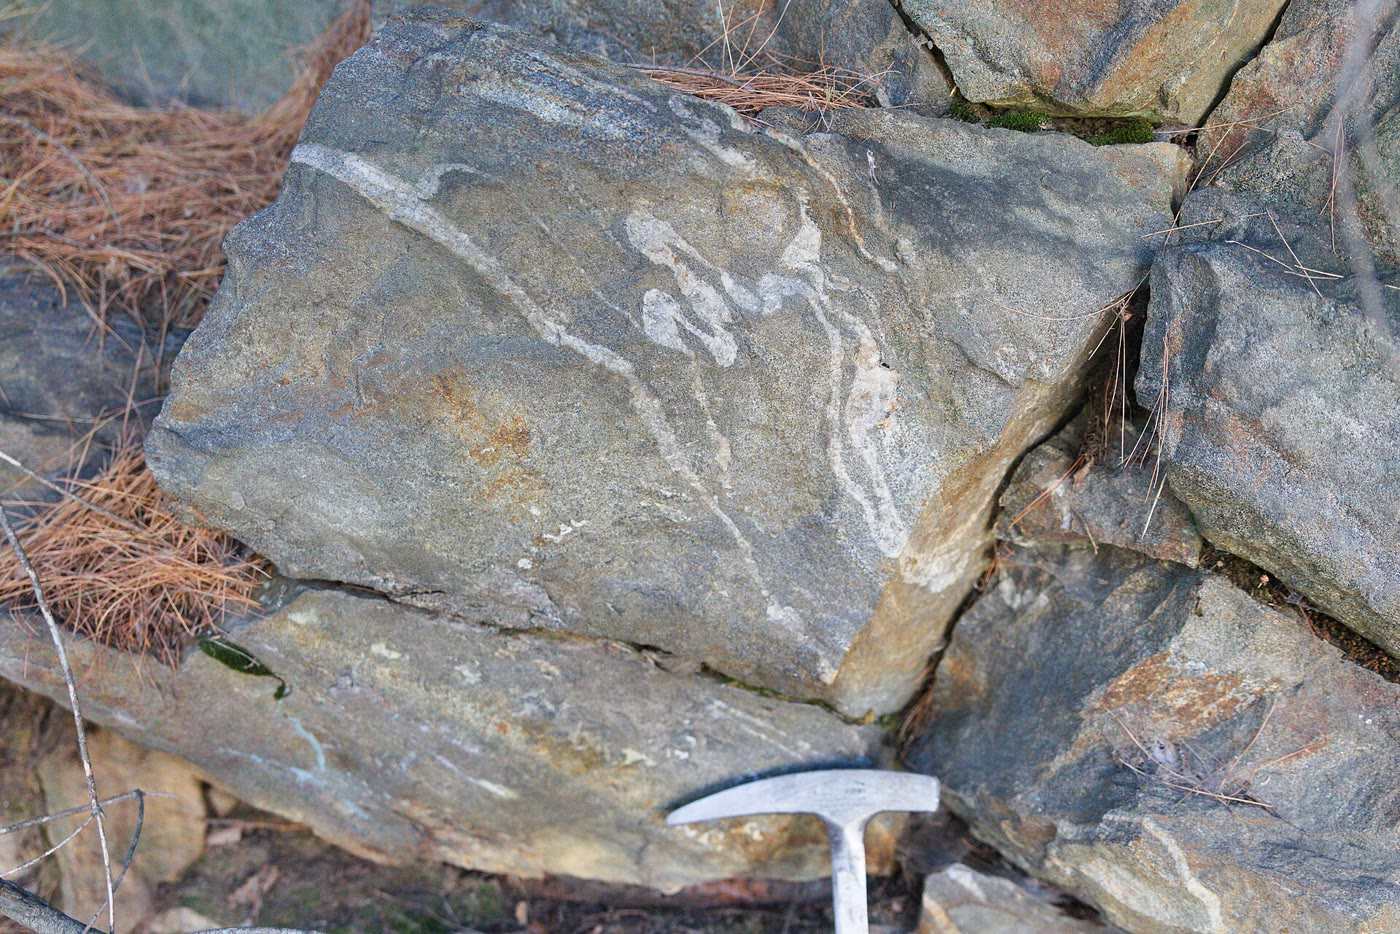
\includegraphics[width=0.62\linewidth]{images/book4/b2-12-migmatite.jpg}
\par\smallskip{\small 新罕布什尔州纳舒厄的一块\omterm{def:b2:crustal-melting:migmatite}{混合岩}：浅色的\omterm{def:b2:crustal-melting:migmatite}{浅色体}脉，
与包裹它们的灰色片麻岩一同褶皱。地质锤提供比例尺。照片：Kevin M. Gill, CC BY 4.0。}
\end{omfigure}

\section{从混合岩到深成岩体}\label{sec:b2:crustal-melting:segregation}

在颗粒尺度上，初始熔体沿颗粒边界分布，并聚集于小熔池中，
主要平行于面理。尽管很小，它却会改变岩石：在对\omterm{def:b2:mantle-melting:melting}{部分熔融}花岗岩的
实验中，集合体的强度在固相线
与\omterm{def:b2:mantle-melting:fraction}{熔体分数} \num{0.07} 之间急剧下降，这是因为含熔体的颗粒边界相互连通，随后
又下降约四个数量级（但起点已很低），当晶体
骨架在更高\omterm{def:b2:mantle-melting:fraction}{熔体分数}下破坏。因此，\omterm{def:b2:mantle-melting:melting}{部分熔融}的地壳较弱，
且一旦熔融开始，变形便集中于此。变形反过来驱动
熔体：它沿相互连锁的颗粒边界从基质中排出，进入
平行于面理的\omterm{def:b2:crustal-melting:migmatite}{浅色体}，再经横切该层的\omterm{def:b2:crustal-melting:migmatite}{浅色体}离开熔融层，并
这些\omterm{def:b2:crustal-melting:migmatite}{浅色体}汇入\cref{ch:b2:magma-emplacement}中的\omterm{def:b2:magma-emplacement:bodies}{岩墙}。下图概括了
从源区到\omterm{def:b2:magma-emplacement:bodies}{深成岩体}的路径。
% ledger: sawyer01:segregation, rh05:connectivity

\begin{omfigure}
\centering
\begin{tikzpicture}[x=1cm, y=1cm]
\fill[gray!20] (0,0) rectangle (11,1.6);
\fill[gray!8] (0,1.6) rectangle (11,5.2);
\node[font=\scriptsize, anchor=west] at (0.1,0.25) {混合岩化下地壳（源区）};
\foreach \x in {0.6,1.6,2.6,3.6,4.6,5.6,6.6,7.6,8.6,9.6} {
  \draw[white, line width=2.2pt] (\x,0.65) .. controls (\x+0.3,0.75) and (\x+0.5,0.6) .. (\x+0.8,0.7);
  \draw[white, line width=2.2pt] (\x+0.2,1.2) .. controls (\x+0.45,1.3) and (\x+0.6,1.15) .. (\x+0.85,1.25);
}
\foreach \x in {2.8, 5.2, 7.9} {
  \draw[red!70!black, line width=1.4pt] (\x,1.3) .. controls (\x+0.1,2.2) and (\x-0.1,2.9) .. (5.5,3.65);
}
\fill[pink!60, draw=red!70!black, thick] (4.0,3.7) .. controls (4.3,4.6) and (6.7,4.6) .. (7.0,3.7)
  .. controls (6.3,3.4) and (4.7,3.4) .. (4.0,3.7);
\node[font=\scriptsize] at (5.5,4.05) {深成岩体};
\node[font=\scriptsize, anchor=west] at (8.3,2.5) {岩墙};
\draw[->, thick] (8.25,2.5) -- (7.95,2.3);
\node[font=\scriptsize, anchor=west] at (0.1,4.85) {上地壳};
\draw[thick] (0,5.2) -- (11,5.2);
\node[font=\scriptsize, anchor=south east] at (10.9,5.2) {地表};
\node[font=\scriptsize, align=left, anchor=west] at (9.0,1.05) {浅色体};
\end{tikzpicture}
\par\smallskip{\small 从\omterm{def:b2:crustal-melting:migmatite}{混合岩}到\omterm{def:b2:magma-emplacement:bodies}{深成岩体}，示意图，未按比例绘制：\omterm{def:b2:crustal-melting:migmatite}{浅色体}
（白色）在\omterm{def:b2:mantle-melting:melting}{部分熔融}源区中汇入\omterm{def:b2:magma-emplacement:bodies}{岩墙}（红色），
为地壳中位置较高的\omterm{def:b2:magma-emplacement:bodies}{深成岩体}供给熔体。}
\end{omfigure}

地壳能保持熔融多久？在喜马拉雅，广泛的\omterm{def:b2:crustal-melting:anatexis}{深熔作用}始于印度与亚洲碰撞之后
约 3000 万年，深熔岩石中的锆石和独居石给出的年龄
约为 2500 万至 1500 万年前；单个样品可能覆盖该时段的大部分。
喜马拉雅地壳的熔融并非一次事件，而是一种
持续约 1000 万年的状态。
% ledger: weinberg16:himalaya

\section{花岗岩类型}\label{sec:b2:crustal-melting:types}

花岗岩的化学成分保留着其源区的信息，首先体现在
它所含铝的量与其长石所能容纳的量相比较。

\begin{definition}[铝饱和指数]\label{def:b2:crustal-melting:asi}
岩石的\emph{铝饱和指数}\index{铝饱和指数}定义为
摩尔比
\[\mathrm{A/CNK} = \frac{n(\ce{Al2O3})}{n(\ce{CaO}) + n(\ce{Na2O}) + n(\ce{K2O})},\]
其伴随量为 $\mathrm{A/NK} = n(\ce{Al2O3})/[n(\ce{Na2O}) + n(\ce{K2O})]$。若岩石
$\mathrm{A/CNK} > 1$，则称为\emph{过铝质}\index{过铝质}，
若 $\mathrm{A/CNK} < 1 < \mathrm{A/NK}$，则称为\emph{准铝质}\index{准铝质}，且
若 $\mathrm{A/NK} < 1$，则称为\emph{过碱性}\index{过碱性}。
\end{definition}
% ledger: moyen17:aluminosity, frost01:asi

\begin{proposition}[指数的含义]\label{prop:b2:crustal-melting:feldspar}
若岩石中的钙、钠和钾全部存在于长石中，且其全部铝也存在于长石中，
则有 $\mathrm{A/CNK} = 1$。因此，\omterm{def:b2:crustal-melting:asi}{过铝质}岩石在长石之外仍剩有
铝，这些铝保存于富铝矿物中（白云母、石榴子石、堇青石、
铝硅酸盐）；\omterm{def:b2:crustal-melting:asi}{准铝质}岩石在长石之外剩有钙，保存于钙硅酸盐中
（角闪石、单斜辉石、榍石）；\omterm{def:b2:crustal-melting:asi}{过碱性}岩石则剩有钠和钾，
保存于铝不足以形成长石的矿物中（钠质辉石和
钠质角闪石）。
\end{proposition}

\begin{proof}
以氧化物形式表示，钾长石为 \ce{K2O.Al2O3.6SiO2}、钠长石为 \ce{Na2O.Al2O3.6SiO2} 而
钙长石为 \ce{CaO.Al2O3.2SiO2}：每个化学式恰含一个 \ce{Al2O3} 与一个
\ce{K2O}、\ce{Na2O} 或 \ce{CaO} 对应。因此，三者的任意混合物均有 $n(\ce{Al2O3}) =
n(\ce{CaO}) + n(\ce{Na2O}) + n(\ce{K2O})$，亦即 $\mathrm{A/CNK} = 1$。若
$\mathrm{A/CNK} > 1$，则铝超过了碱金属和钙所能结合进长石的量，
多余的铝必须存在于其他矿物中。若 $\mathrm{A/CNK} < 1$ 但
$\mathrm{A/NK} > 1$，则铝足以使全部钠和钾形成长石，
但不足以使全部钙形成长石，多余的钙进入
每个钙所需铝少于钙长石的矿物中。若 $\mathrm{A/NK} < 1$，则即使碱金属也不能全部进入
长石。
\end{proof}

莫延等人发现，在区分源区不同的花岗岩时，铝度是最有用的
指标；弗罗斯特等人使用同一指数，并对磷作小幅校正，
将其作为花岗质
岩石分类三个坐标轴之一。
% ledger: moyen17:aluminosity, frost01:asi

\begin{omfigure}
\centering
\begin{tikzpicture}
\begin{axis}[omrecord, width=0.72\linewidth, height=7cm,
  xmin=0.4, xmax=1.5, ymin=0.4, ymax=3.5, xlabel={A/CNK（摩尔比）}, ylabel={A/NK（摩尔比）},
  tick label style={font=\scriptsize}, label style={font=\small}]
\addplot[fill=gray!15, draw=none] coordinates {(0.4,0.4) (1.5,1.5) (1.5,0.4) (0.4,0.4)};
\addplot[thick, black!70] coordinates {(1,0.4) (1,3.5)};
\addplot[thick, black!70] coordinates {(0.4,1) (1.5,1)};
\node[font=\scriptsize, anchor=north east] at (axis cs:1.48,3.45) {过铝质};
\node[font=\scriptsize, anchor=west] at (axis cs:0.62,2.6) {准铝质};
\node[font=\scriptsize, anchor=south west] at (axis cs:0.42,0.45) {过碱性};
\addplot[only marks, mark=*, mark size=2pt, blue!70!black, nodes near coords,
  point meta=explicit symbolic, every node near coord/.style={font=\scriptsize, anchor=west}]
  coordinates {(0.539,3.196)[BHVO-2] (0.877,1.694)[AGV-2] (0.993,1.135)[SRM 278]};
\addplot[only marks, mark=square*, mark size=2pt, red!70!black]
  coordinates {(1.261,1.377) (0.809,0.844)};
\node[font=\scriptsize, red!70!black, anchor=south] at (axis cs:1.261,1.45) {S 型熔体};
\node[font=\scriptsize, red!70!black, anchor=north] at (axis cs:0.809,0.79) {过碱性花岗岩};
\end{axis}
\end{tikzpicture}
\par\smallskip{\small 尚德图。蓝色圆圈：三种参考物质，即夏威夷
玄武岩（BHVO-2）、安山岩（AGV-2）以及花岗质成分的黑曜岩（SRM 278），
依据其已发表的氧化物含量计算得出。红色方块：本章所用的两种
虚构花岗岩。灰色三角形无法到达，因为 A/CNK 从不超过 A/NK。}
\end{omfigure}
% ledger: usgs:bhvo2-major, usgs:agv2-major, nist278:majors

化学成分随源岩而定。1974 年，查佩尔与怀特注意到，除
长英质程度最高的岩石外，Lachlan 褶皱带的花岗岩可分为两个截然不同的组，
并将其解释为两类源岩熔融的产物：较老的火成岩与沉积岩。长石的水解作用在本科一年级
分册中已见过，它使钠与钙以溶液形式被带走，并使铝保留在黏土中：由这些黏土形成的泥
质沉积物富含铝，其熔体同样富铝。
% ledger: cw01:is-types

\begin{definition}[花岗岩类型学]\label{def:b2:crustal-melting:types}
称 \emph{I 型花岗岩}\index{I 型花岗岩}为源区主要为
较老火成岩的花岗岩，称 \emph{S 型花岗岩}\index{S 型花岗岩}为源区主要为
沉积（变沉积）岩的花岗岩，称由地幔衍生的花岗岩为 M 型花岗岩。
\emph{A 型花岗岩}\index{A 型花岗岩}不依其源区定义，而依其化学性质与
构造环境定义：富铁、富钾，强烈富集\omterm{def:b2:elements-in-the-earth:partition}{不相容元素}，
并侵位于稳定的板内、弧后或碰撞后环境中。
\end{definition}
% ledger: johansson23:a-type, cw01:is-types

\omterm{def:b2:crustal-melting:types}{S 型花岗岩}呈\omterm{def:b2:crustal-melting:asi}{过铝质}，含两种云母或堇青石；A 型花岗质岩石
多为\omterm{def:b2:crustal-melting:asi}{准铝质}，部分为\omterm{def:b2:crustal-melting:asi}{过铝质}。然而，单个分析可能产生误导：每个花岗质岩套都
终结于花岗岩最低点附近的成分，贫暗色矿物且略呈\omterm{def:b2:crustal-melting:asi}{过铝质}，
故\omterm{def:b2:crustal-melting:asi}{过铝质}样品并不能证明地壳曾经熔融。区分各岩套的是
其在尚德图中的轨迹形态：弧岩套
沿陡峭趋势带自高 A/NK、低 A/CNK 处到达最低点，低钙 S 型岩套
则沿 A/NK 接近 A/CNK 的趋势带到达最低点。关于 A 型\omterm{def:b2:magma-emplacement:magma}{岩浆}的来源尚无共识：
一种模型认为，它们源自底侵玄武岩，经结晶分异、
\omterm{def:b2:mantle-melting:melting}{部分熔融}及\omterm{def:b2:magmatic-differentiation:open}{地壳同化}作用而演化形成。
% ledger: moyen17:trends, frost01:asi, johansson23:a-type

\begin{definition}[淡色花岗岩]\label{def:b2:crustal-melting:leucogranite}
\emph{淡色花岗岩}\index{淡色花岗岩}为一种浅色花岗岩，几乎不含
暗色矿物；碰撞带的\omterm{def:b2:crustal-melting:asi}{过铝质}淡色花岗岩含白云母，单独或
与黑云母共存。
\end{definition}
% ledger: moyen17:aluminosity, pdh98:himalaya

碰撞带中含白云母的\omterm{def:b2:crustal-melting:asi}{过铝质}\omterm{def:b2:crustal-melting:leucogranite}{淡色花岗岩}，其成分接近含水或白云母\omterm{def:b2:crustal-melting:reactions}{脱水熔融}所得的液相，
温度接近
\qty{700}{\celsius}，此时源区中的锆石与独居石仍可存留，并以捕获晶形式进入熔体；
含堇青石的\omterm{def:b2:crustal-melting:asi}{过铝质}花岗岩则来自
黑云母在更高温度下的分解，温度为 800 至 \qty{850}{\celsius}。喜马拉雅\omterm{def:b2:crustal-melting:leucogranite}{淡色花岗岩}，
凭其强烈的地壳同位素特征，属于这一类岩石，
（见\cref{ch:b2:himalaya-andes}）。
% ledger: moyen17:aluminosity, weinberg16:himalaya

\begin{omfigure}
\centering
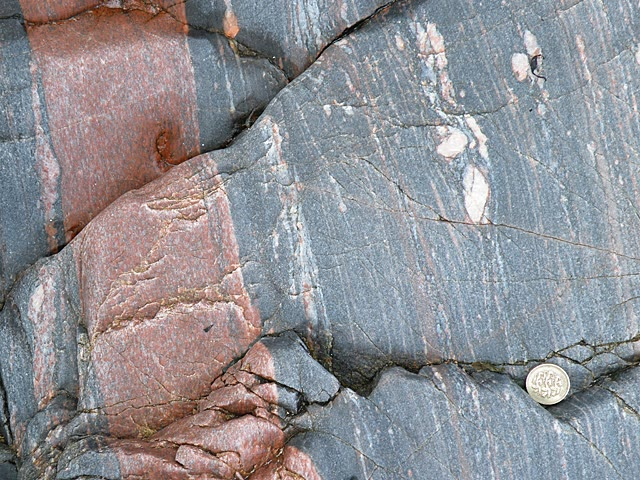
\includegraphics[width=0.5\linewidth]{images/book4/b2-12-leucogranite-vein.jpg}
\par\smallskip{\small 粉红色\omterm{def:b2:crustal-melting:leucogranite}{淡色花岗岩}脉切穿带状灰色片麻岩，硬币给出
比例尺。照片：Anne Burgess (Geograph), CC BY-SA 2.0。}
\end{omfigure}

\section{花岗岩与大陆的生长}\label{sec:b2:crustal-melting:time}

地球上多数花岗岩形成于两类环境。在俯冲带之上，弧地壳通过
地幔镁铁质熔体的分异作用形成，此时可用的热量仅来自这些
熔体所带来的热量。碰撞之后，加厚的地壳是一个极热的体系，它大规模地熔融，
在有水或白云母时于较低温度下，在较高温度下
靠黑云母分解，这些源自地壳的花岗岩再循环了
已存在的地壳。地幔熔体也在此处抵达地壳，其量足够大，据莫延等人
的观点，晚造山带将成为地壳生长的重要贡献者。因此，花岗岩究竟是增加
大陆还是仅改造大陆，取决于其源区，
这可由同位素加以判定（见\cref{ch:b2:isotope-geochemistry}）；早期地球的花岗岩
与此截然不同，是
\cref{ch:b2:precambrian-earth}的主题。
% ledger: moyen17:settings

\section{练习}\label{sec:b2:crustal-melting:exercises}

摩尔质量（\unit{\gram\per\mole}）：\ce{Al2O3} 101.96，\ce{CaO} 56.08，\ce{Na2O} 61.98，
\ce{K2O} 94.20，\ce{H2O} 18.02；原子质量：H 1.008，O 16.00，Na 22.99，Mg 24.31，
Al 26.98，Si 28.09，K 39.10，Ca 40.08。取 $g = \qty{9.81}{\metre\per\second\squared}$。

\begin{exercise}[$\star$]\label{exo:b2:crustal-melting:1}
安山岩参考物质 AGV-2 中，以 \unit{\gram} 每 \qty{100}{\gram} 计，含
\ce{Al2O3} 17.03，\ce{CaO} 5.15，\ce{Na2O} 4.204 和 \ce{K2O} 2.898。
（a）计算其 A/CNK 与 A/NK。（b）对其分类，并指出一种应容纳其
过剩钙的矿物。
\end{exercise}
% ledger: usgs:agv2-major

\begin{exercise}[$\star$]\label{exo:b2:crustal-melting:2}
除石英和长石外，三种花岗岩还含有：（a）白云母、黑云母和石榴子石；
（b）普通角闪石、黑云母和榍石；（c）霓石，一种钠–铁辉石
\ce{NaFeSi2O6}，以及一种钠质角闪石。依其\omterm{def:b2:crustal-melting:asi}{铝饱和指数}对每种花岗岩分类，并说明
哪一种可能是 \omterm{def:b2:crustal-melting:types}{S 型花岗岩}。
\end{exercise}

\begin{exercise}[$\star$]\label{exo:b2:crustal-melting:3}
地壳密度为 \qty{2800}{\kilogram\per\cubic\metre}，其地温线为线性
：$T = \qty{10}{\celsius} + (\qty{20}{\celsius\per\kilo\metre})\,z$。在 2 与
\qty{10}{kbar} 之间，以过
(\qty{680}{\celsius}, \qty{2}{kbar}) 与 (\qty{620}{\celsius}, \qty{10}{kbar}) 两点的直线近似湿花岗岩的固相线。求地温线与之相交处的
深度、温度与压强。
\end{exercise}
% ledger: sw81:wet-solidus

\begin{exercise}[$\star$]\label{exo:b2:crustal-melting:4}
一块灰色黑云母片麻岩中含有厘米厚的白色石英与长石层，这些层与其面理平行，
每层两侧各以一条薄的黑云母暗色条带为界；层间的片麻岩看来普通。
（a）说出白色层、黑色条带与普通片麻岩的名称。
（b）该岩石是\omterm{def:b2:crustal-melting:migmatite}{变熔混合岩}还是\omterm{def:b2:crustal-melting:migmatite}{深熔混合岩}？其构造如何？（c）相距数百
米之外，层理已经消失：一种条纹状、类似花岗岩的岩石中保留着片麻岩的
微弱残影。发生了什么变化？
\end{exercise}
% ledger: scmr:migmatite, bgs99:migmatite

\begin{exercise}[$\star\star$]\label{exo:b2:crustal-melting:5}
取黑云母为金云母 \ce{KMg3AlSi3O10(OH)2}。（a）计算其摩尔质量，及它所释放的
水的质量分数（其两个羟基给出一个 \ce{H2O}）。（b）一块黑云母
（按质量计）占 \qty{25}{\percent} 的片麻岩经黑云母\omterm{def:b2:crustal-melting:reactions}{脱水熔融}，生成含水
\qty{4.0}{\percent} 的熔体。利用
\cref{prop:b2:crustal-melting:water}，求\omterm{def:b2:mantle-melting:fraction}{熔体分数}，并将其与
黑云母\omterm{def:b2:crustal-melting:reactions}{脱水熔融}实验中所得的\omterm{def:b2:mantle-melting:fraction}{熔体分数}相比较。
\end{exercise}
% ledger: bk99:migmatites

\begin{exercise}[$\star\star$]\label{exo:b2:crustal-melting:6}
一百克花岗岩中含 \qty{30}{\gram} 钾长石 \ce{KAlSi3O8}，
\qty{35}{\gram} 钠长石 \ce{NaAlSi3O8}，\qty{5}{\gram} 钙长石 \ce{CaAl2Si2O8}，
\qty{25}{\gram} 石英和 \qty{5}{\gram} 白云母 \ce{KAl3Si3O10(OH)2}。
（a）计算四种含铝矿物的摩尔质量。（b）计算
岩石中 \ce{Al2O3}、\ce{CaO}、\ce{Na2O} 和 \ce{K2O} 的物质的量，并求其 A/CNK。（c）哪种
矿物使该岩石成为\omterm{def:b2:crustal-melting:asi}{过铝质}？
\end{exercise}

\begin{exercise}[$\star\star$]\label{exo:b2:crustal-melting:7}
一块在 \qty{1200}{\celsius} 侵入的玄武质岩席完全结晶，并冷却至
\qty{850}{\celsius}，同时释放 \qty{900}{\mega\joule\per\cubic\metre} 的潜热。
其周围温度为 \qty{650}{\celsius} 的地壳被加热至 \qty{850}{\celsius}，
其中 \qty{20}{\percent} 发生熔融，熔体单位体积的潜热与上相同。两种
岩石的热容均为 \qty{2.5}{\mega\joule\per\cubic\metre\per\kelvin}。
由\cref{prop:b2:crustal-melting:heat}可知，一立方米
玄武岩能以此方式处理多少立方米地壳？该结果忽略了什么？
\end{exercise}
% ledger: delaney86b4:properties

\begin{exercise}[$\star\star$]\label{exo:b2:crustal-melting:8}
黑曜岩参考物质 SRM 278 的认定含量为 \ce{Al2O3}
$14.15 \pm 0.15$，\ce{CaO} 0.983，\ce{Na2O} 4.84 和 \ce{K2O} 4.16（均为 \unit{\percent}，
质量分数）。（a）计算其 A/CNK 与 A/NK，并进行分类。（b）分别用
\ce{Al2O3} 不确定度的两个端值重新计算 A/CNK。该分类是否稳健？
\end{exercise}
% ledger: nist278:majors

\begin{exercise}[$\star\star$]\label{exo:b2:crustal-melting:9}
在 \qty{800}{\celsius} 下，被水饱和的二长花岗质熔体
在 \qty{3}{kbar} 时含水 \qty{7.45}{\percent}，在 \qty{4}{kbar} 时为 8.94，在 \qty{5}{kbar} 时为 9.97，在
\qty{8}{kbar} 时为 13.82。（a）用最小二乘法对这四个点拟合直线，并
将其斜率与实验者给出的每千巴 \qty{1.27}{\percent} 相比较。
（b）预测 \qty{6}{kbar} 时的饱和含量。（c）在 \qty{6}{kbar} 下能携带
\qty{10}{\gram} 水的熔体最小质量是多少？（d）为何该直线不应
用于 \qty{15}{kbar}？
\end{exercise}
% ledger: holtz95:solubility

\begin{exercise}[$\star\star\star$]\label{exo:b2:crustal-melting:10}
用直线近似白云母片岩的\omterm{def:b2:crustal-melting:reactions}{脱水熔融}固相线，
该直线通过（\qty{750}{\celsius}，\qty{6}{kbar}）和（\qty{800}{\celsius}，\qty{10}{kbar}）两点，
这两点为实验括号的端点。一块温度为 \qty{770}{\celsius} 的片岩从
\qty{10}{kbar} 开始上升，且不吸热也不放热。（a）它在何种压强下到达
固相线？（b）此后，其温度沿固相线下降，熔融所需的热量
来自其自身冷却。已知热容为 \qty{2.5}{\mega\joule\per\cubic\metre\per\kelvin}，
潜热为 \qty{900}{\mega\joule\per\cubic\metre}，求其到达
\qty{6}{kbar} 时已形成的熔体体积分数？（c）与为
喜马拉雅\omterm{def:b2:crustal-melting:leucogranite}{淡色花岗岩}提出的条件进行比较。
\end{exercise}
% ledger: pdh98:himalaya, delaney86b4:properties

\begin{exercise}[$\star\star\star$]\label{exo:b2:crustal-melting:11}
热量扩散过距离 $\ell$，时间量级为 $\ell^2/\kappa$。取
$\kappa = \qty{1e-6}{\square\metre\per\second}$，估算
\qty{2}{km} 厚岩席与 \qty{10}{km} 厚底侵层的热量，
扩散到各自厚度所需的时间。与喜马拉雅\omterm{def:b2:crustal-melting:anatexis}{深熔作用}的一千万年相比较：一次
底侵事件能否解释它？
\end{exercise}
% ledger: delaney86b4:properties, weinberg16:himalaya

\begin{exercise}[$\star\star\star$]\label{exo:b2:crustal-melting:12}
一块条带状\omterm{def:b2:crustal-melting:migmatite}{混合岩}经分析：\omterm{def:b2:crustal-melting:migmatite}{浅色体} \ce{K2O} \qty{5.0}{\percent}，\ce{MgO}
\qty{0.20}{\percent}；\omterm{def:b2:crustal-melting:migmatite}{暗色体} \ce{K2O} \qty{2.0}{\percent}，\ce{MgO}
\qty{4.0}{\percent}；中色体（视为未熔化的母体），\ce{K2O}
\qty{2.75}{\percent}，\ce{MgO} \qty{3.05}{\percent}（均为质量分数）。（a）若
新成体由母体形成且无物质增减，则其中\omterm{def:b2:crustal-melting:migmatite}{浅色体}的质量分数为
多少？（b）用 \ce{MgO} 检验该结果。（c）在露头上，\omterm{def:b2:crustal-melting:migmatite}{浅色体}仅占
新成体质量的 \qty{10}{\percent}。每
\qty{100}{\gram} 母岩中，留下的熔体有多少克？
\end{exercise}

\begin{problem}[{周末问题——由熔融云母形成的深成岩体}]\label{pb:b2:crustal-melting:1}
一块由 \qty{20}{\percent} 白云母、\qty{15}{\percent} 黑云母、
\qty{30}{\percent} 石英、\qty{30}{\percent} 斜长石和 \qty{5}{\percent} 其他
矿物组成的片岩（质量分数；为虚构岩石）位于经叠置而加厚一倍的地壳底部，
即在\cref{ch:b2:pt-paths}中建模的情形。该岩石可能熔融，并为花岗岩\omterm{def:b2:magma-emplacement:bodies}{深成岩体}提供熔体。数据：
练习开头给出的原子量与摩尔质量；湿花岗岩固相线经过
（\qty{680}{\celsius}，\qty{2}{kbar}）、（\qty{620}{\celsius}，\qty{10}{kbar}）、
（\qty{605}{\celsius}，\qty{15.3}{kbar}）和（\qty{670}{\celsius}，\qty{27}{kbar}）；
花岗质熔体在 \qty{800}{\celsius} 下的水饱和含量：\qty{9.97}{\percent}（\qty{5}{kbar}）、
\qty{13.82}{\percent}（\qty{8}{kbar}）。加厚地壳的模型底部如下：

\smallskip
\begin{center}\small
\begin{tabular}{l|ccccccccccc}
$t$ (\unit{Ma}) & 0 & 10 & 20 & 30 & 40 & 50 & 60 & 70 & 80 & 90 & 100\\ \hline
$T$ (\unit{\celsius}) & 595 & 656 & 734 & 795 & 845 & 885 & 909 & 914 & 900 & 867 & 814\\
$P$ (\unit{kbar}) & 19.2 & 19.2 & 19.2 & 19.2 & 17.9 & 16.5 & 15.1 & 13.7 & 12.4 & 11.0 & 9.6
\end{tabular}
\end{center}
\smallskip

\noindent\textbf{第一部分——云母中的水。}
\begin{enumerate}
\item 计算白云母 \ce{KAl3Si3O10(OH)2} 的摩尔质量。
\item 其两个羟基生成一个 \ce{H2O}。该矿物有多大质量分数以水的形式
释放？
\item 一千克片岩中的白云母会释放多少水？
\item 线性插值，求熔体在
\qty{7}{kbar} 时的饱和含水量。则白云母的水至少能产生的最小\omterm{def:b2:mantle-melting:fraction}{熔体分数}为多少？
\item \omterm{def:b2:crustal-melting:reactions}{脱水熔融}的熔体远未饱和，取其含水量为
\qty{6.0}{\percent}。白云母能产生多少\omterm{def:b2:mantle-melting:fraction}{熔体分数}？
\item 在 \qty{10}{kbar} 下对双云母\omterm{def:b2:metamorphic-facies:protoliths}{变泥质岩}的实验中，白云母反应
仅产生 1 至 \qty{2}{\percent} 的熔体。试给出真实岩石可能产生的熔体少于
你对第~5 题答案的两个原因。
\end{enumerate}

\noindent\textbf{第二部分——加热源岩。}
\begin{enumerate}[resume]
\item 在\cref{ch:b2:pt-paths}中，留在地壳中部的岩石峰值为 \qty{593}{\celsius}
和 \qty{7.8}{kbar}。\qty{7.8}{kbar} 时的湿固相线为多少？该岩石
即使有自由水，能否熔融？
\item 在 15.3 与 \qty{27}{kbar} 之间插值，求
叠置刚结束时底部压强处的湿固相线。在 $t = 0$ 时，底部温度是否高于它？在 $t = \qty{10}{Ma}$ 时呢？
\item 是什么限制了 $t = \qty{10}{Ma}$ 时底部的熔融，以及它为何
很快停止？
\item 底部何时越过 \qty{800}{\celsius}，即白云母
括号的上端？
\item 角闪石括号跨越 875 至 \qty{925}{\celsius}，压强为 \qty{10}{kbar} 至 \qty{12.5}{kbar}。
底部何时进入该压强范围，以及进入时的温度为多少？
\item 底部何时达到 \qty{10}{kbar}，即白云母实验压强范围的上限，
此时温度多高？片岩中哪些含水矿物仍能
存在？
\end{enumerate}

\noindent\textbf{第三部分——何种熔体？}
熔体一旦结晶，便得到一种\omterm{def:b2:crustal-melting:leucogranite}{淡色花岗岩}（虚构分析），其成分（按
\unit{\percent} 质量计）为：\ce{Al2O3} 15.0、\ce{CaO} 0.55、\ce{Na2O} 3.4 和 \ce{K2O} 4.9。
\begin{enumerate}[resume]
\item 计算岩石中 \qty{100}{\gram} 内四种氧化物的物质的量。
\item 计算其 A/CNK。
\item 计算其 A/NK，并对该\omterm{def:b2:crustal-melting:leucogranite}{淡色花岗岩}进行分类。
\item 它是 I 型还是 \omterm{def:b2:crustal-melting:types}{S 型花岗岩}？写出两种应容纳其过剩
铝的矿物。
\item 长石消耗后，每 \qty{100}{\gram} 岩石中还剩余
多少摩尔的 \ce{Al2O3}？若全部进入白云母，白云母每个化学式单元比钾长石多
一个 \ce{Al2O3}，则 \qty{100}{\gram} 花岗岩中
将含白云母多少克？
\item 黑曜岩 SRM 278 的 A/CNK $= 0.993$。\omterm{def:b2:crustal-melting:leucogranite}{淡色花岗岩}与该黑曜岩
是否可能来自同一类源区？
\end{enumerate}

\noindent\textbf{第四部分——有多少地壳？}
一个虚构的该\omterm{def:b2:crustal-melting:leucogranite}{淡色花岗岩}\omterm{def:b2:magma-emplacement:bodies}{深成岩体}，体积为 \qty{1000}{\cubic\kilo\metre}。
取花岗岩的密度为 \qty{2650}{\kilogram\per\cubic\metre}，
片岩的密度为 \qty{2800}{\kilogram\per\cubic\metre}；假设熔体的 \qty{70}{\percent} 离开
其源区，且熔体结晶时其全部水分均逸出。
\begin{enumerate}[resume]
\item 该\omterm{def:b2:magma-emplacement:bodies}{深成岩体}的质量是多少？
\item 形成该\omterm{def:b2:magma-emplacement:bodies}{深成岩体}需要多少质量的熔体（含 \qty{6.0}{\percent} 水）？
\item 利用第~5 题的\omterm{def:b2:mantle-melting:fraction}{熔体分数}，需要熔融多少质量的片岩？
\item 该片岩的体积是多少？
\item 若源区为厚 \qty{5}{km} 的岩层，则熔融所覆盖的面积为多少？
\item 若改用第~4 题中的最小\omterm{def:b2:mantle-melting:fraction}{熔体分数}，源区需
大多少？给出形成该\omterm{def:b2:magma-emplacement:bodies}{深成岩体}所熔融的源区地壳体积，
单位为 \unit{\cubic\kilo\metre}（取自第~22 题）。
\end{enumerate}
\end{problem}
